% ============================================================================
% Slides de defesa — TCC: Geração de Música por IA Generativa
% Beamer (LaTeX). Compila com pdflatex (2x).
% Imagens necessárias na mesma pasta (4): figura_metricas.png, figura_comparacao.png,
% figura_mos.png, slide_colapso.png
% (slide_modelo_puro.png é backup opcional do demo — não referenciado nos slides)
%
% No Overleaf: New Project -> Blank, cole este arquivo, suba as imagens acima.
% ============================================================================
\documentclass[aspectratio=169]{beamer}

\usepackage[utf8]{inputenc}
\usepackage[brazil]{babel}
\usepackage{amsmath}
\usepackage{graphicx}
\usepackage{tikz}
\usetikzlibrary{arrows.meta, positioning}

\usetheme{Madrid}
\usecolortheme{whale}
\setbeamertemplate{navigation symbols}{}
\setbeamertemplate{caption}[numbered]

% Cores
\definecolor{azulT}{RGB}{21,101,192}
\definecolor{vermelhoM}{RGB}{198,40,40}

\title[Geração de Música por IA]{Geração de Música por Meio de\\Inteligência Artificial Generativa}
\author[Lucas Ikeda]{Lucas Vinícius de Carvalho Ikeda}
\institute[UNESP]{Orientador: Prof.\ Dr.\ Danillo Roberto Pereira\\Faculdade de Ciências e Tecnologia --- UNESP}
\date{Defesa de TCC --- 2026}

\begin{document}

% ---------- Slide 1: Capa ----------
\begin{frame}
  \titlepage
\end{frame}

% ---------- Slide 2: Problema e Objetivo ----------
\begin{frame}{Problema e Objetivo}
  \begin{block}{Objetivo central}
    Gerar uma peça em formato \texttt{.mid} que um \textbf{humano reconheça como
    música} --- mesmo simples --- e \textbf{não confunda com ruído aleatório}.
  \end{block}
  \vspace{0.4em}
  \begin{itemize}
    \item O critério de sucesso é, no fundo, \textbf{perceptual}.
    \item Por isso a avaliação final é feita com \textbf{ouvintes humanos} (MOS).
    \item A saída deve ser compatível com qualquer DAW (MuseScore, FL Studio).
  \end{itemize}
\end{frame}

% ---------- Slide 3: Por que é difícil ----------
\begin{frame}{Por que é difícil?}
  Música exige \textbf{coordenar quatro dimensões ao mesmo tempo}:
  \begin{columns}[T]
    \begin{column}{0.5\textwidth}
      \begin{itemize}
        \item \textbf{Melódica} --- notas no tempo
        \item \textbf{Harmônica} --- acordes
      \end{itemize}
    \end{column}
    \begin{column}{0.5\textwidth}
      \begin{itemize}
        \item \textbf{Rítmica} --- padrões temporais
        \item \textbf{Tímbrica} --- qual instrumento
      \end{itemize}
    \end{column}
  \end{columns}
  \vspace{1em}
  \begin{alertblock}{O desafio}
    Não é gerar notas --- é gerar notas \textbf{coordenadas} e com coerência de
    longo prazo. Modelos neurais sozinhos tendem a colapsar ou ``perder o tempo''.
  \end{alertblock}
\end{frame}

% ---------- Slide 4: Fundamentação ----------
\begin{frame}{Fundamentação: \emph{Transformer} + Tokenização}
  \begin{columns}[T]
    \begin{column}{0.58\textwidth}
      \textbf{\emph{Transformer}} (a base do ChatGPT) usa \textbf{atenção} para
      capturar dependências longas:
      \[
        \mathrm{Attention}(Q,K,V)=\mathrm{softmax}\!\left(\frac{QK^{T}}{\sqrt{d_k}}\right)V
      \]
      \footnotesize Processa toda a sequência em paralelo, sem o gargalo das RNNs.
    \end{column}
    \begin{column}{0.42\textwidth}
      \textbf{Tokenização REMI}\\
      Trata música como linguagem:
      \begin{itemize}\footnotesize
        \item \texttt{NOTE\_ON}, \texttt{NOTE\_OFF}
        \item \texttt{VELOCITY}, \texttt{TIME\_SHIFT}
        \item \texttt{BAR}, \texttt{BEAT} (estrutura métrica)
      \end{itemize}
    \end{column}
  \end{columns}
\end{frame}

% ---------- Slide 5: Trabalhos Relacionados ----------
\begin{frame}{Trabalhos Relacionados}
  \begin{itemize}
    \item \emph{Music Transformer} e \emph{Pop Music Transformer} --- mostraram que
      \emph{Transformers} capturam regularidades musicais.
    \item \emph{MuseGAN} (GANs), \emph{MusicVAE} (VAE), \emph{DeepBach} (restrições
      harmônicas).
  \end{itemize}
  \vspace{0.8em}
  \begin{block}{A lacuna que preencho}
    Fazer funcionar com \textbf{recursos modestos} (uma GPU de 8\,GB),
    \textbf{combinando a rede neural com teoria musical}.
  \end{block}
\end{frame}

% ---------- Slide 6: Visão Geral (pipeline) ----------
\begin{frame}{Visão Geral: um sistema híbrido}
  \begin{center}
  \resizebox{\textwidth}{!}{%
  \begin{tikzpicture}[
    box/.style={rectangle, rounded corners, draw=azulT, very thick,
      fill=azulT!10, minimum height=1.1cm, text width=2.3cm, align=center},
    teoria/.style={rectangle, rounded corners, draw=vermelhoM, very thick,
      fill=vermelhoM!10, minimum height=1.1cm, text width=2.3cm, align=center},
    arr/.style={-{Stealth[length=3mm]}, very thick}]
    \node[box](d){Datasets MIDI};
    \node[box, right=0.7cm of d](t){Tokenização REMI};
    \node[box, right=0.7cm of t](m){\emph{Transformer} (treino)};
    \node[teoria, right=0.7cm of m](c){\emph{Constrained Decoding}};
    \node[teoria, below=0.7cm of c](v){Separação de vozes};
    \node[box, left=0.7cm of v](o){MIDI final};
    \draw[arr](d)--(t); \draw[arr](t)--(m); \draw[arr](m)--(c);
    \draw[arr](c)--(v); \draw[arr](v)--(o);
  \end{tikzpicture}}
  \end{center}
  \vspace{0.5em}
  \begin{center}
    \textbf{A ideia-chave:} o \textcolor{azulT}{modelo aprende}, e a
    \textcolor{vermelhoM}{teoria musical dá os trilhos}.
  \end{center}
\end{frame}

% ---------- Slide 7: Modelo + Dados ----------
\begin{frame}{Modelo e Dados}
  \begin{columns}[T]
    \begin{column}{0.5\textwidth}
      \textbf{Modelo (compacto)}
      \begin{itemize}\footnotesize
        \item \emph{Decoder-only} (estilo GPT)
        \item \textbf{3,2 milhões} de parâmetros
        \item d\_model 256, 4 camadas, 4 cabeças
        \item Cabe em \textbf{8\,GB} de VRAM (AMP)
      \end{itemize}
    \end{column}
    \begin{column}{0.5\textwidth}
      \textbf{Dados (3 \emph{datasets})}
      \begin{itemize}\footnotesize
        \item \emph{MAESTRO} --- piano clássico
        \item \emph{POP909} --- pop multi-voz
        \item \emph{Groove} --- bateria humana
      \end{itemize}
    \end{column}
  \end{columns}
  \vspace{1em}
  \footnotesize\textit{Modelo menor generaliza melhor em bases de tamanho moderado
  --- e o gargalo não era tamanho, era calibração da perda.}
\end{frame}

% ---------- Slide 8: Mode collapse -> label smoothing ----------
\begin{frame}{O problema do \emph{mode collapse} (e a solução)}
  \begin{columns}[c]
    \begin{column}{0.5\textwidth}
      \begin{itemize}\small
        \item O modelo \textbf{travava} numa díade fixa após dezenas de notas.
        \item Diagnóstico: \textbf{\emph{overconfidence}} no \texttt{TIME\_SHIFT}.
        \item Solução: \textbf{\emph{label smoothing}} (0,1) --- mantém incerteza
          saudável.
        \item Foi a intervenção que \textbf{destravou} os resultados.
      \end{itemize}
      \footnotesize\textit{Gargalo era calibração da perda, não o tamanho do modelo.}
    \end{column}
    \begin{column}{0.5\textwidth}
      \centering
      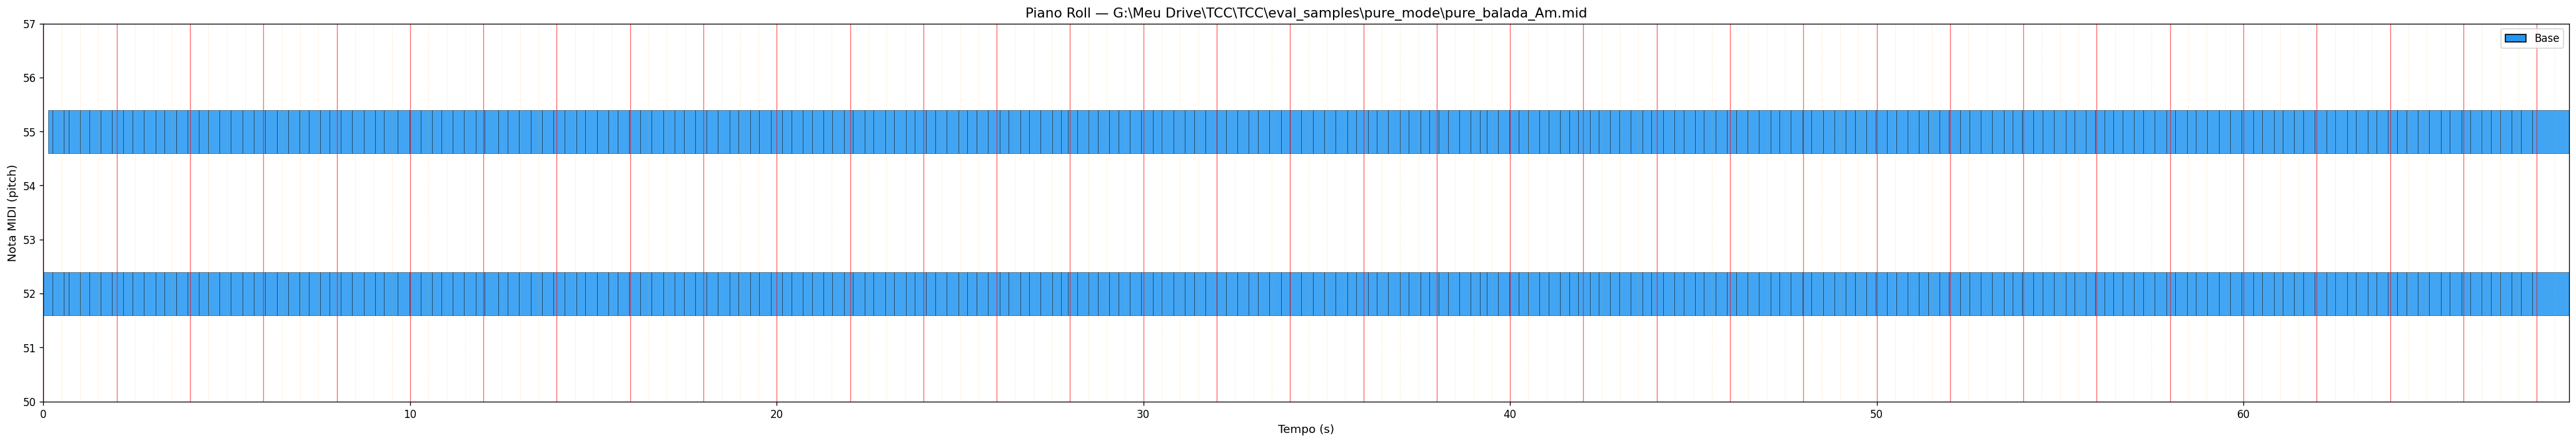
\includegraphics[width=\textwidth]{slide_colapso.png}\\
      \tiny Exemplo de colapso: duas notas fixas por toda a peça.
    \end{column}
  \end{columns}
\end{frame}

% ---------- Slide 9: Geração com restrições ----------
\begin{frame}{Geração com Restrições (\emph{Constrained Decoding})}
  Quatro estágios que guiam a amostragem sem substituir o modelo:
  \begin{enumerate}
    \item \textbf{Restrições de vocabulário} --- gramática + harmonia da tonalidade.
    \item \textbf{\emph{Re-entry bias}} --- ``convite'' para a voz calada voltar.
    \item \textbf{Separação de vozes} por registro (solo / base / baixo).
    \item \textbf{Fundação harmônica} opcional (\texttt{--solid\_base}) --- robustez.
  \end{enumerate}
  \vspace{0.5em}
  \begin{block}{}
    \centering As restrições \textbf{não criam} a música --- elas \textbf{direcionam}
    o que o modelo aprendeu para regiões coerentes.
  \end{block}
\end{frame}

% ---------- Slide 10: Resultados Quantitativos ----------
\begin{frame}{Resultados Quantitativos --- \emph{Transformer} vs Markov}
  \begin{columns}[c]
    \begin{column}{0.62\textwidth}
      \centering
      
\includegraphics[width=\textwidth]{figura_metricas.png}
    \end{column}
    \begin{column}{0.38\textwidth}
      \begin{itemize}\small
        \item Markov ``vence'' algumas métricas --- mas porque \textbf{copia}
          trechos do \emph{dataset}.
        \item Na \textbf{regularidade rítmica} (\emph{ioi\_std}) o sistema vence
          com folga: \textbf{0,17 vs 0,32}.
        \item Métrica isolada não mede musicalidade $\Rightarrow$ MOS é o juiz.
      \end{itemize}
    \end{column}
  \end{columns}
\end{frame}

% ---------- Slide 11: Qualitativo + Demo ----------
\begin{frame}{Resultados Qualitativos + Demonstração}
  \begin{columns}[c]
    \begin{column}{0.5\textwidth}
      \centering
      
\includegraphics[width=\textwidth]{figura_comparacao.png}\\
      \tiny \emph{Transformer} (acima): 3 camadas. Markov (abaixo): disperso.
    \end{column}
    \begin{column}{0.5\textwidth}
      \begin{itemize}\small
        \item \emph{Transformer}: três camadas coordenadas (solo, base, baixo).
        \item Markov: dispersão sem função nem fundação rítmica.
      \end{itemize}
      \vspace{0.5em}
      \begin{alertblock}{\small Demonstração (áudios)}
        \footnotesize Markov (caos) $\rightarrow$ \textbf{modelo sozinho}
        $\rightarrow$ sistema completo. \textbf{[tocar trechos]}
      \end{alertblock}
    \end{column}
  \end{columns}
\end{frame}

% ---------- Slide 12: Resultados do MOS ----------
\begin{frame}{Avaliação Subjetiva (MOS) --- $N = 25$ avaliadores}
  \begin{center}
    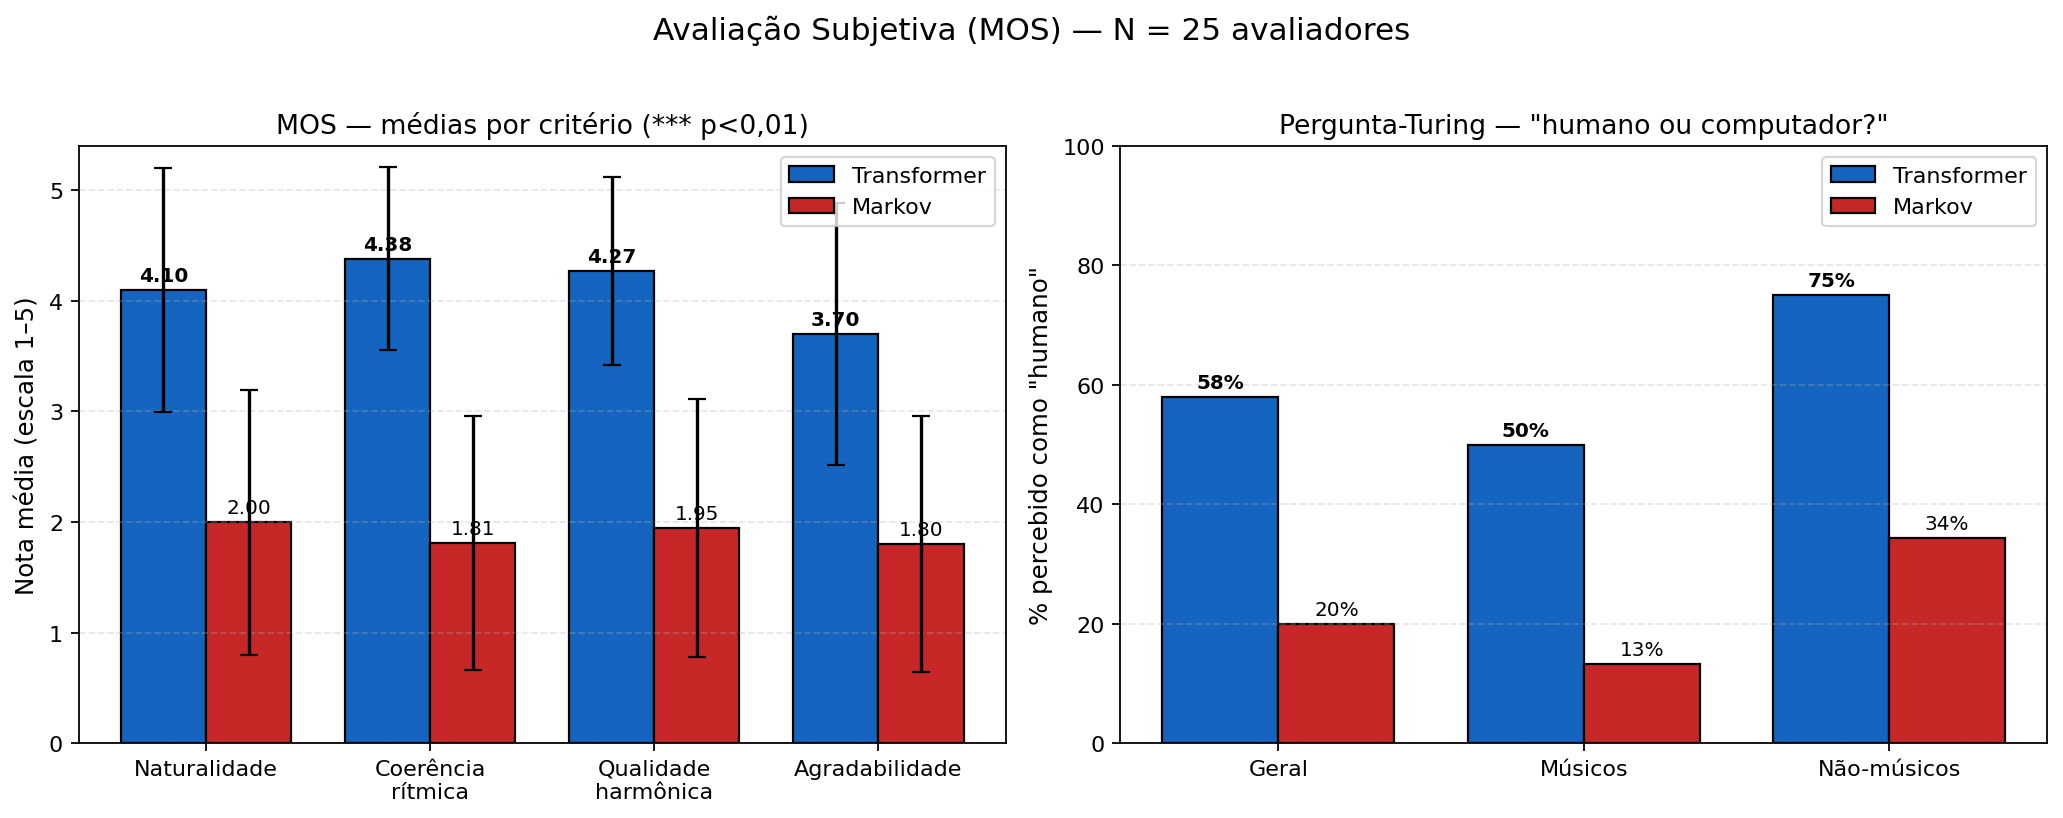
\includegraphics[width=0.96\textwidth]{figura_mos.png}
  \end{center}
  \vspace{0.2em}
  \begin{center}\small
    O \textbf{\emph{Transformer} vence os 4 critérios} ($p < 0{,}01$) e é percebido
    como \textbf{humano por 58\%} dos avaliadores --- contra 20\% do Markov.
  \end{center}
\end{frame}

% ---------- Slide 13: Conclusão ----------
\begin{frame}{Conclusão}
  \begin{itemize}
    \item \textbf{Critério atendido e validado:} a saída é reconhecida como música
      por ouvintes humanos --- confirmado pelo MOS ($p < 0{,}01$), em nítido
      contraste com o caos do Markov.
    \item \textbf{Contribuição:} um \emph{pipeline} híbrido (rede neural $+$ teoria
      musical) que roda em hardware modesto, com diagnóstico e solução do
      \emph{mode collapse}.
    \item \textbf{Trabalhos futuros:} modelo dedicado de bateria; condicionamento
      por estilo; comparação com modelos maiores.
  \end{itemize}
\end{frame}

% ---------- Slide 14: Obrigado ----------
\begin{frame}[plain]
  \begin{center}
    {\Huge Obrigado!}\\[1em]
    {\large Perguntas?}\\[2em]
    \small Lucas Vinícius de Carvalho Ikeda\\
    \texttt{l.ikeda@unesp.br}
  \end{center}
\end{frame}

\end{document}
